\documentclass[tikz,border=2pt]{standalone}
\usepackage{amsmath,amssymb}
\usepackage{tikz}
\usetikzlibrary{arrows.meta}

\begin{document}
% Five observations in the order they were drawn (top) and sorted (bottom): the k-th order
% statistic X_(k) is the k-th smallest value, so X_(1) is the minimum and X_(5) the maximum.
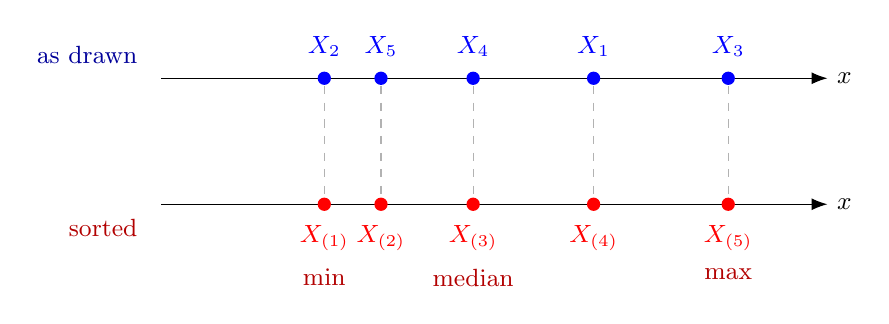
\begin{tikzpicture}[x=0.9cm, every node/.style={font=\small}, >={Latex[length=2mm]}]
	\draw[->] (0,0) -- (9.4,0) node[right] {$x$};
	\foreach \x/\i in {6.1/1, 2.3/2, 8.0/3, 4.4/4, 3.1/5} {
		\fill[blue] (\x,0) circle (2.4pt);
		\node[blue, anchor=south] at (\x,0.15) {$X_{\i}$};
	}
	\node[blue!60!black, anchor=east] at (-0.2,0.3) {as drawn};
	\draw[->] (0,-1.6) -- (9.4,-1.6) node[right] {$x$};
	\foreach \x/\k in {2.3/1, 3.1/2, 4.4/3, 6.1/4, 8.0/5} {
		\fill[red] (\x,-1.6) circle (2.4pt);
		\node[red, anchor=north] at (\x,-1.75) {$X_{(\k)}$};
		\draw[gray!60, dashed] (\x,-0.1) -- (\x,-1.5);
	}
	\node[red!70!black, anchor=east] at (-0.2,-1.9) {sorted};
	\node[red!70!black, anchor=north] at (2.3,-2.3) {min};
	\node[red!70!black, anchor=north] at (8.0,-2.3) {max};
	\node[red!70!black, anchor=north] at (4.4,-2.3) {median};
	
\end{tikzpicture}
\end{document}
